\documentclass[a4j,12pt]{gradthesis_utf8}
%\usepackage[dviout]{graphicx}
\usepackage[dvipdfmx]{graphicx}
\usepackage{graphicx}
%
%%% ドラフトモード(図表は,図表のみのページになる)
%\draftmode
%
%%% 2ページ目に英語の題目をいれる
\engtitle
%
%%% 2ページ目に英語の所属をいれる
\engaffil
%
%%% 2ページ目に英語の著者名をいれる
\engauthor
%
%%% ヘッダ(章番号と章タイトル)を入れる
\usehead
%
\jtitle{TCP並列接続を用いたプログレッシブダウンロード\\における順序制御方式の実装} % 和文題目
%
\etitle{Implementation of sequence control method in progressive download using TCP parallel connection} % 英文題目
%
\jaffil{広島市立大学 情報科学部 情報工学科}
\eaffil{Department of Computer and Network Engineering\\
Faculty of Information Sciences\\
Hiroshima City University}
%
\jauthor{1420180 \quad 平城 光雄} % 和文著者名
\eauthor{1420180 \quad Mitsuo Heijo} % 英文著者名
\supervisor{舟坂 淳一}  % 指導教官名
%
%
\jabst{ % 和文梗概 
\hspace*{0.5em}概要
} %

\eabst{ % 英文梗概
\hspace*{1em}gaiyo}

\begin{document} 
\maketitle %とびらの出力

%%%%%%%%%%%%%%%%%%%%%%%%%%%%%%%%%%%%%%%%%%%%%%%%%%%%%%%%%%%%%%%%%%%%%%%%%%%%%
% 第1章
%%%%%%%%%%%%%%%%%%%%%%%%%%%%%%%%%%%%%%%%%%%%%%%%%%%%%%%%%%%%%%%%%%%%%%%%%%%%%
\chapter{はじめに}\label{sec:sec1}
%%% abst %%%
はじめに
%%%%%%%%%%%%%%%%%%%%%%%%%%%%%%%%%%%%%%%%%%%%%%%%%%%%%%%%%%%%%%%%%%%%%%%%%%%%%
% 第2章
%%%%%%%%%%%%%%%%%%%%%%%%%%%%%%%%%%%%%%%%%%%%%%%%%%%%%%%%%%%%%%%%%%%%%%%%%%%%%
\chapter{関連研究}\label{sec:sec2}
本章ではまず,動画配信方式の一つであるプログレッシブダウンロードについて述べる.

\section{プログレッシブダウンロード方式}
ネットワークの大容量化,高速化に伴い,Youtube[]やNetflix[]などの動画配信サービスの利用が増加している.動画配信サービスにはUDPを利用したストリーミング,TCPを利用したプログレッシブダウンロードの2種類がある.アプリケーションプロトコルとしてHTTPを用いるプログレッシブダウンロードは特別なソフトウェアを必要とせず,ブラウザだけで視聴することができるため,近年広く普及してきている.また,プログレッシブダウンロードは分割順次ダウンロードとも呼称される.\\
プログレッシブダウンロードの動作概要は,まず,1つのファイルを複数のあるサイズののブロックに分割する.次に,クライアントは分割されたブロックをサーバーに対してリクエストする.このリクエストの方法にはHTTPのRange Headerに分割のための情報を含める方式やHTTPのGETリクエストのクエリストリングに分割のための情報を含める方式などがある.サーバーはリクエストに応じたブロックを送信する.これを繰り返すことで,1つのファイルを取得できる.

%%%%%%%%%%%%%%%%%%%%%%%%%%%%%%%%%%%%%%%%%%%%%%%%%%%
%%%%%%%%%%%%%%%%%%%%%%%%%%%%%%%%%%%%%%%%%%%%%%%%%%%
 \section{複数経路を用いた通信方式}
 複数のIP接続を束ねて上位層に機能を提供することを目的としたものの一つのMPTCP[]などが提案されている.複数のNICを束ねることで上位層からは1つの仮想的なインターフェースとして扱うことができる.これらは各OSレベルでの実装が必要となるので実装コストが高い.
 

%%%%%%%%%%%%%%%%%%%%%%%%%%%%%%%%%%%%%%%%%%%%%%%%%%%%%%%%%%%%%%%%%%
 \section{複数のTCP接続を用いたプログレッシブダウンロード}
 ネットワークの発展に伴い,大容量のデータをTCPを用いて,通信する機会が増加しつつある.TCPには輻輳回避のためにウィンドウ制御が存在する.このため,ウィンドウサイズを遅延で割ったものが単一TCP接続における理論最大性能となる.近年ではコンテンツの大容量化が進んでおり,より効率よくコンテンツをダウンロードするためにアプリケーション層から複数のTCP接続を用いる手法が提案されている.\\
 \ref{block}は複数のTCPを接続を用いたプログレッシブダウンロードの分割されたブロックの受信の様子を示した例である。複数のブロックを別々のTCP接続に対して要求を行う場合,ブロックの再生順番と受信完了順序が一致しない可能性がある.図..が示すように,先頭から連続するブロック1及びブロック2は再生可能である(有効ブロック)が,それ以降のブロック..は未受信のブロックを間に挟んでいるため再生することはできない(非有効ブロック).複数のTCP接続を束ねることでグッドプットを向上させても,受信ブロックが有効ブロックでない限りは応答性は低下してしまい,ユーザー体験は悪化することが予想できる.先行研究ではこの問題への解決作として
\begin{figure}[h]
\centering
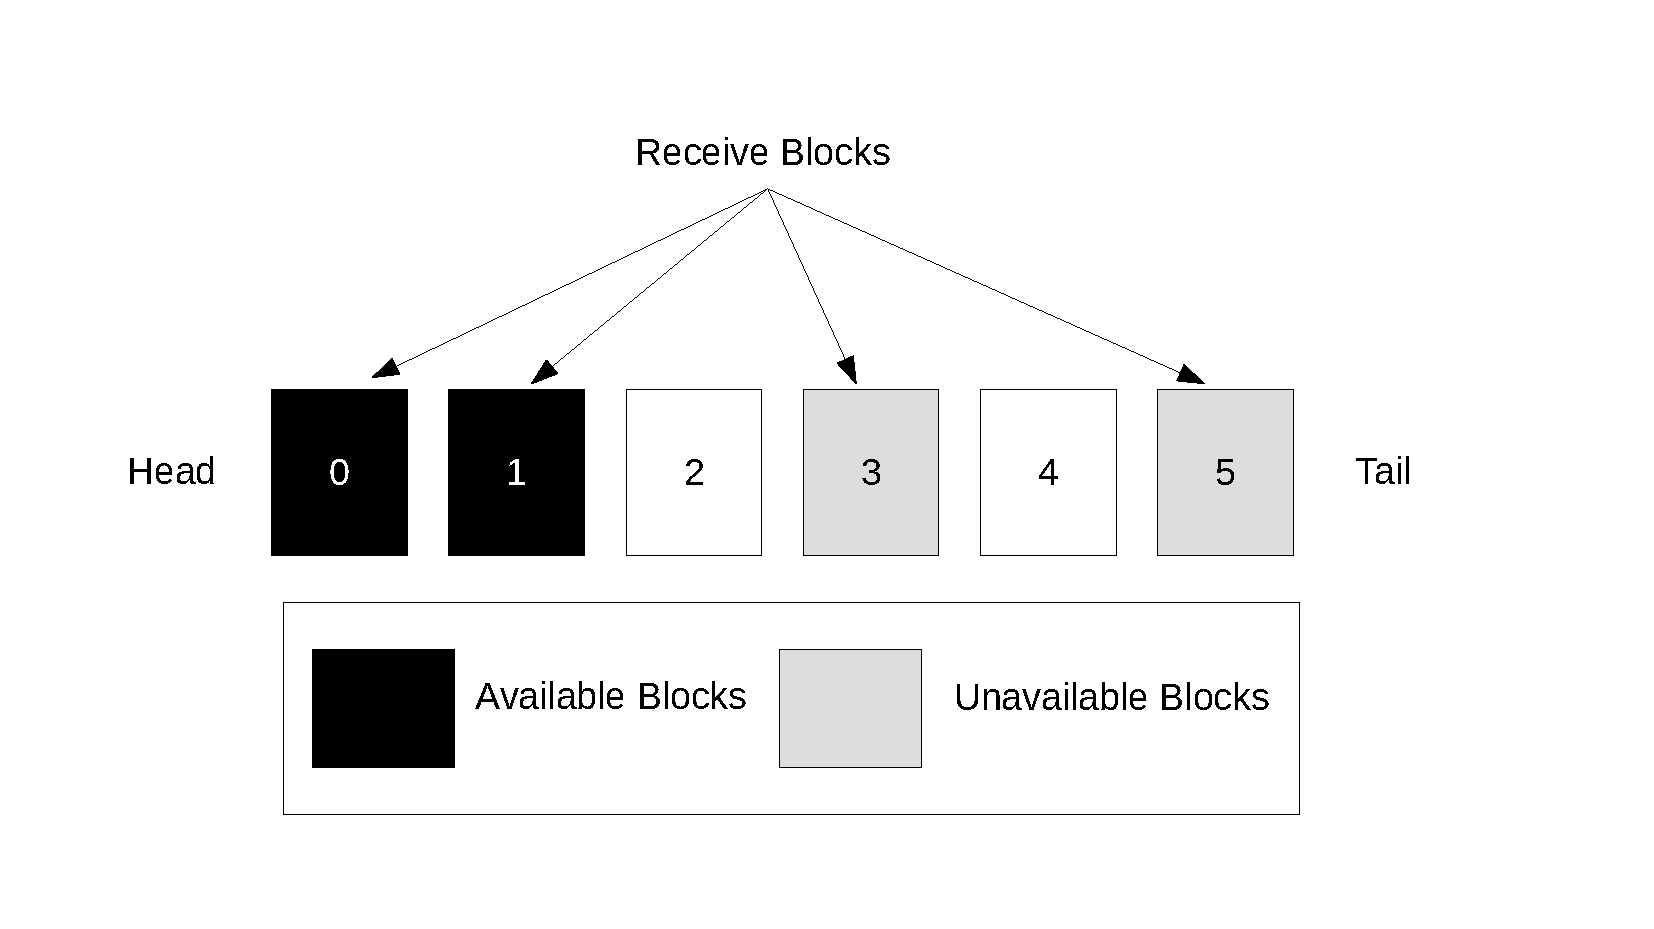
\includegraphics[width=18cm]{block.pdf}
\caption{ブロックの有効性}
\label{block}
\end{figure}
 %%%%%%%%%%%%%
 
 \section{タイマ駆動を用いた要求方式}
 
\chapter{提案方式}\label{sec:sec3}
本章では性能差のある複数のTCP接続を並列的に利用する際に生じうるいくつかの問題点を解消するためのアルゴリズムを実装した提案方式について述べる。\\
また,実際に複数のTCP接続を用いた動画のプログレッシブダウンロードをプログラムに実装する際に考慮すべき点がいくつかある。プログレッシブダウンロードの実装は大きく分けて動画ファイルのダウンロードとバイナリファイルをデコードして再生という2つのセクションに分かれている。既存のウェブブラウザやVLC[]等のネットワークメディア再生機能付きの動画プレイヤーソフトのではこの2つのセクションは1つのプログラムから高度に同期をとりながら同時並列的に制御されている。しかし、本研究では実装の難易度と主としてダウンロードセクションについて論じるためにこれら2つのセクションは分離している。
\section{遅延要求方式}
\subsection{固定遅延方式}

\subsection{差分計測を用いた遅延予測方式}

\subsection{接続使用回数比を用いた遅延予測方式}

\section{重複再要求方式}
\subsection{バッファ内非有効ブロック数依存方式}
\subsection{非有効ブロック受信回数依存方式}

\chapter{実装評価}\label{sec:sec4}

\section{提案方式の評価}
\subsection{テストベッドでの評価}

\subsection{実ネットワークでの評価}
実ネットワークでの評価にあたりUbuntuのパブリックミラーサーバーを利用した.\\
使用したサーバー群
\begin{table}[htb]
	\begin{tabular}{lll}
		ホスト & 組織 & 国\\
		ftp.jaist.ac.jp & JAIST & JP \\
		ubuntutym2.u-toyama.ac.jp & Univercity of Toyama & JP \\
		releases.ubuntu.com & Canonical & GB \\
		mirrorservice.org & University of Kent & GB \\
		ubuntu.ipacct.com & IPACCT & BG \\
		mirror.enzu.com & Enzu Inc. & US \\
		mirror.pop-sc.rnp.br & PoP-SC & BR \\
		ftp.belnet.be & Belnet & BE \\
		mirrors.mit.edu & MIT & US \\
		mirror.yandex.ru & Yandex & RU \\
	\end{tabular}
\end{table}

参考 各サーバーの24時間の性能の時間変化
\begin{figure}
	\begin{center}
		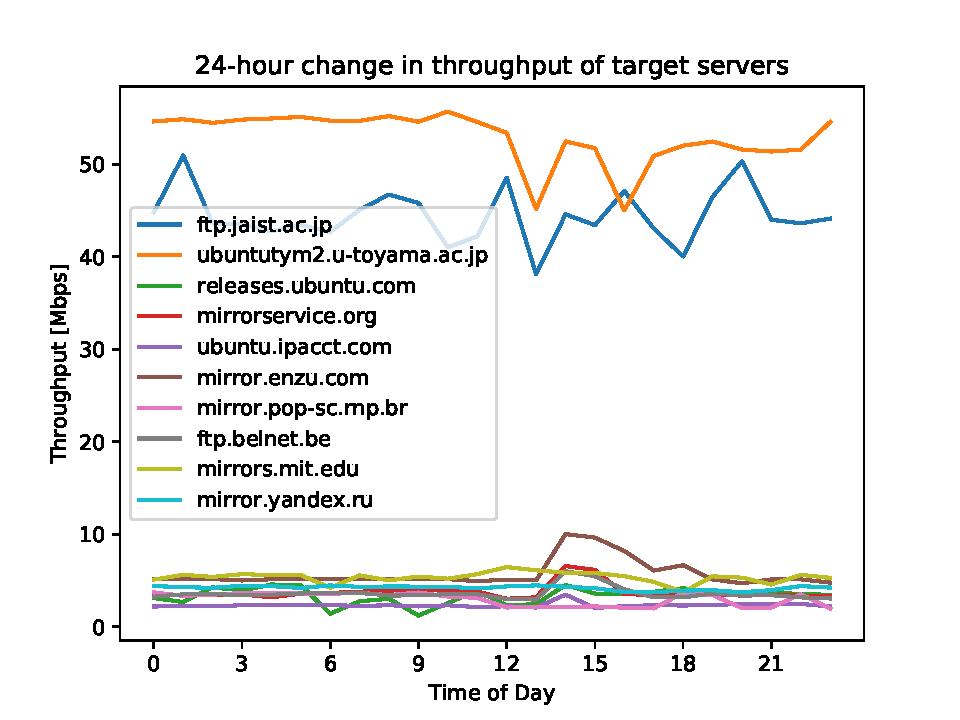
\includegraphics[width=15cm]{thp24h.pdf}
	\end{center}
\end{figure}


\chapter{動画配信サーバーへの適用例}
\section{プロキシでの実装}
 
%%%%%%%%%%%%%%%%%%%%%%%%%%%%%%%%%%%%%%%%%%%%%%%%%%%%%%%%%%%%%%%%%%%%%%%%%%%%
% 第X章
%%%%%%%%%%%%%%%%%%%%%%%%%%%%%%%%%%%%%%%%%%%%%%%%%%%%%%%%%%%%%%%%%%%%%%%%%%%%%
\chapter{今後の課題}\label{sec:sec7}
\hspace*{0.5em}今後の課題として, 以下が挙げられる.
\begin{itemize}
	\item 実際のユーザー体験を考慮した評価
	\item タイマ駆動要求方式の実装との比較
\end{itemize}
\clearpage
%
%%%%%%%%%%%%%%%%%%%%%%%%%%%%%%%%%%%%%%%%%%%%%%%%%%%%%%%%%%%%%%%%%%%%%%%%%%%%%
% 謝辞
%%%%%%%%%%%%%%%%%%%%%%%%%%%%%%%%%%%%%%%%%%%%%%%%%%%%%%%%%%%%%%%%%%%%%%%%%%%%%
\begin{acknowledgment}
 本研究の機会を与えて頂き,多くの御指導,および御助言を賜わりました
舟坂 淳一 准教授に深甚なる謝意を表します.また,その他多くの御助言を頂きま
した諸氏に心より感謝致します.
\end{acknowledgment}
%%%%%%%%%%%%%%%%%%%%%%%%%%%%%%%%%%%%%%%%%%%%%%%%%%%%%%%%%%%%%%%%%%%%%%%%%%%%%
% 参考文献
%%%%%%%%%%%%%%%%%%%%%%%%%%%%%%%%%%%%%%%%%%%%%%%%%%%%%%%%%%%%%%%%%%%%%%%%%%%%%
\begin {thebibliography}{20} 
\bibitem{test} test

\end {thebibliography}

\end{document}
